\documentclass{article}
\usepackage{amsmath}
\usepackage{amsthm}
\usepackage{graphicx}
\usepackage{tcolorbox}
\usepackage{lmodern}
\usepackage{titling}
\usepackage{quoting}
\usepackage{mathrsfs}
\usepackage{mathtools}
\usepackage{etoolbox}
\usepackage{amsfonts}
\usepackage{hyperref}
\usepackage{tikz}
\usepackage[a4paper,
            bindingoffset=0.2in,
            left=0.5in,
            right=0.5in,
            top=1in,
            bottom=1in]{geometry}
\hypersetup{hidelinks}
\makeatletter
\newenvironment{chapquote}[2][2em]
  {\setlength{\@tempdima}{#1}%
   \def\chapquote@author{#2}%
   \parshape 1 \@tempdima \dimexpr\textwidth-2\@tempdima\relax%
   \itshape}
  {\par\normalfont\hfill--\ \chapquote@author\hspace*{\@tempdima}\par\bigskip}
\makeatother
\linespread{1.618}
\quotingsetup{vskip=6pt}
\tcbuselibrary{theorems}
\newtcolorbox[auto counter, number within=subsection]{defin}[1]{
fonttitle=\bfseries, title=Definition~\thetcbcounter: #1}
\newtcolorbox[auto counter, number within=subsection]{thm}[1]{colframe = blue!75!black!200, colback = blue!5,
fonttitle=\bfseries, title=Theorem~\thetcbcounter: #1}
\newtcolorbox[auto counter, number within= subsection]{lemma}[1]{colframe =
green!70!black!200, colback = green!5, fonttitle = \bfseries, title=Lemma~\thetcbcounter: #1}
\begin{document}
\begin{titlepage}
    \begin{center}
        \vspace{8cm}
        % Title
        {\fontsize{30}{30}\bfseries Algebra and Analysis} \\
        \vspace{0.5cm}
        % Author and date information
        \textbf{Yuxin Gong} \\
        \vfill

        \normalsize{Imperial College London} \\

    \end{center}
\end{titlepage}
\tableofcontents
\newpage
\section{Mathematical logic}
\begin{chapquote}{David Hilbert}
    ``Wir müssen wissen. Wir werden wissen.''
\end{chapquote}
\subsection{Proposition and logic}
\quad\ Before introducting the first definition, making sure what are common expressions,
here are some examples:
\begin{itemize}
    \item Mathematics is a good subject
    \item $\pi$
    \item $1 + 1$
\end{itemize}
\quad\ The first expression is ambiguous, how to define what is a ``\textbf{good}'' subject? The
second and third one are just some items in the Math. But in the world of Math, one can
not deal with those ``non-sense'' things. We need definitions!!
\begin{defin}{Proposition}
        A proposition is a declarative statement that is either true or false
        but not both.
\end{defin}
This means that if someone gives you a proposition in mathematics, it can be either true or
false. Once you encounter expresssions like this:
\begin{center}
    \textbf{This proposition is False.}
\end{center}
\quad\  
You will realize this is no longer a proposition anymore. If it is true, then it is false. If it is
false, then it is true. You should do this three times by yourself, you will realize that this is impossible
a proposition.\\
\subsection{More about propositions}
\quad There will also be some cases that the second proposition is related to the first proposition.
Now a truth table is needed to record the T/F value of those two propositions. This note will not include
formal definition of a truth table as it is a technical thing to do when combining several propositions.
\subsubsection{AND (Conjunction)}
\quad\ Suppose that $P$ and $Q$ are propositions. In our real life, we always say both something and something
are true. When it comes to mathematics, it becomes \textbf{AND}. Denoting \textbf{AND} as $\land$, $P \land Q$
becomes a new proposition. Now it's time to use truth table!!\\
\begin{defin}{AND $\land$}
    Truth table for conjunction is summarized as follows:
\begin{center}
\begin{tabular}{|c|c|c|}
    \hline
    $P$ & $Q$ & $P \land Q$ \\ \hline
    T   & T  & T  \\ \hline
    T   & F  & F  \\ \hline
    F   & T  & F  \\ \hline
    F   & F  & F  \\ \hline
\end{tabular}
\end{center}
\end{defin}
\subsubsection{OR (Disjunction)}
\quad\ Similarly, denoting \textbf{OR} as $\lor$. To connect those concepts with real life, you can actually
think about a real life example. A familiy is expecting to have two children, the first proposition is that the
elder child is boy, the second proposition is that the younger child is boy. Now if we combine those two propositions
using an OR logic connective. The proposition will be one of the children is boy. Think about this yourself.
\begin{defin}{OR $\lor$}
    Truth table for disjunction is summarized as follows:
\begin{center}
\begin{tabular}{|c|c|c|}
    \hline
    $P$ & $Q$ & $P \land Q$ \\ \hline
    T   & T  & T  \\ \hline
    T   & F  & T  \\ \hline
    F   & T  & T  \\ \hline
    F   & F  & F  \\ \hline
\end{tabular}
\end{center}
\end{defin}
\subsubsection{NOT (Negation)}
\quad\ Negation is one of most famous logic connective you will use in your daily life. You can think every proposition you make in
your daily life and work with its negation.
\begin{defin}{NOT $\neg$}
    Truth table for negation is summarized as follows:
\begin{center}
\begin{tabular}{|c|c|c|}
    \hline
    $P$ & $\neg P$ \\ \hline
    T   & F   \\ \hline
    F   & T  \\ \hline

\end{tabular}
\end{center}
\end{defin}
By definition, one can say that either a proposition is true or its negation is true.
\subsubsection{IMPLIES}
\quad\ This is the connective that most people will get confused with at first. Just imagine, we will
have four cases in this situation. How can we define $P\implies Q$ in each stage? First, we give
the definition of it and explain it later.
\begin{defin}{IMPLIES $\implies$}
    Truth table for implies is summarized as follows:
    \begin{center}
    \begin{tabular}{|c|c|c|}
        \hline
        $P$ & $Q$ & $P \implies Q$ \\ \hline
        T   & T  & T \\ \hline
        T   & F  & F \\ \hline
        F   & T  & T \\ \hline
        F   & F  & T \\ \hline
    \end{tabular}
    \end{center}
\end{defin}
Think carefully about this. Taking a mathematical\footnote{We haven't introduced what is $x$, what is $y$, even what is $1$!!} example,
let $P$ to be $x=y$ and let $Q$ to be $a\times x = a \times y$, given
all $x$, $y$, $a$ are real numbers. In mathematical logic, one knows that $P \implies Q$ is True. From the table, this means
$Q$ must be True if $P$ is True. To convince ourselves that the third row and forth row are correct, try $x = 1$, $y = 2$ and $a = 0$ and
$x = 1$, $y = 2$ and $a = 1$.
\subsubsection{Logical equivalence}
\quad\ Logical equivalence has symbol $\iff$. In below, ``$\coloneqq$'' means defined to be.
\begin{defin}{EQUIVALENCE $\iff$}
    $P \iff Q \coloneqq (P \implies Q)\land (Q \implies P)$

\end{defin}
You can construct a truth table for $\iff$.
\begin{center}
    \begin{tabular}{|c|c|c|c|c|}
        \hline
        $P$ & $Q$ & $P \implies Q$ & $Q \implies P$ & $Q \iff P$\\ \hline
        T   & T   & T & T  & T\\ \hline
        T   & F   & F & T  & F\\ \hline
        F   & T   & T & F  & F\\ \hline
        F   & F   & T & T  & T \\ \hline
    \end{tabular}
\end{center}
\quad\ This means once you know $P \iff Q$ is True, then $P$ and $Q$ are going to have same T/F value.
\subsection{Basic laws in logic}
\quad\ You should be able to prove the following lemmas by yourself. Here, when we say ``then $Q$'', this means that
the proposition $Q$ is True.
\begin{lemma}

    Given $P$ a proposition, then $\neg (\neg P) \iff P$.

\end{lemma}
Hint: Run all the possibilities in a truth table, check they have the same value.
\begin{thm}{De Morgan's Law}
    Suppose that $P$ and $Q$ are propositions, then:
\begin{itemize}
    \item[1.] $\neg (P \land Q) \iff (\neg P) \lor (\neg Q)$
    \item[2.] $\neg (P \lor Q) \iff (\neg P) \land (\neg Q)$
\end{itemize}
\end{thm}
Hint: your proof should include a truth table with $8$ columns.
\begin{lemma}{Equivalent definition}
    $(P \implies Q) \iff (\neg P) \lor Q$\\
    $P \lor (Q \land \neg Q) \iff P$\\
    $(P \iff Q) \iff \neg (P \lor Q) \lor (P \land Q)$

\end{lemma}
\subsubsection{Properties in implication}
\quad\ You might use the following relation in your real life already, consider three propositions $P$, $Q$ and $R$. If
$P$ can imply $Q$ and $Q$ can imply $R$, almost all the people will think that $P$ can imply $R$.
This is also true in mathematical logic, try to prove the following lemma.
\begin{lemma}{Transitivity in implication}
$(P \implies Q) \land (Q \implies R) \implies (P \implies R)$
\end{lemma}
You now have at least two ways to prove this result when distributivity of $\lor$ and $\land$ are introduced later.
\begin{lemma}{Contrapositive}
    $(P \implies Q) \iff (\neg Q \implies \neg P)$
\end{lemma}
Think about how useful this result can be when we are doing math!! For example, if it is difficult to argue the statement
forwards, this is a probably a way to think ``backwards''.
\begin{lemma}{Distributivity}
    Suppose that $P$,$Q$ and $R$ are propositions, now:
    \begin{itemize}
        \item[1.] $P \land (Q \lor R) \iff (P \land Q) \lor (P \land R)$
        \item[2.] $P \lor (Q \land R) \iff (P \lor Q) \land (P \lor R)$
    \end{itemize}

\end{lemma}
It has a high degree of symmetry, you can remember the formula easily by recognizing it.
\subsection{Quantifiers}
\quad\ Usually quantifiers are introduced with the logic, however, it would be better to define ``set''. Most common quantifiers are ``$\exists$'' and ``$\forall$''.
$\exists$ means there exists at least, usually in a set. $\forall$ means for all, usually means for all elements in a set.
\subsection{Examples and Practice:}
\quad\ Here will be an example to illustrate how the mathematical logic related to our daily proof.
\begin{itemize}
    \item[\textbf{Q1.}] Prove that if $n$ is an integer, then $n$ is even if and only if $n^2$ is even.(\textit{Imperial IUM Course Example})
\end{itemize}
Here is my explaination, let $P$ be the proposition $n$ is even and $Q$ be the proposition that
$n^2$ is even. Our goal is to prove that $P \iff Q$ is always true. By definition, that is to prove
$P \implies Q$ and $Q \implies P$ are both true. Basic idea is to find some intermediate proposition,
e.g. $P_1$, $P_2 \cdots P_n$. Then by transitivity $(P\implies P_1) \land (P_1 \implies P_2) \implies (P \implies P_2)$,
if one knows that $P \implies P_1$ is true and $P_1 \implies P_2$ is true, then $P \implies P_2$ must be
true. Follow this idea, proving that $P \implies Q$ is true, so is $Q \implies P$.
\begin{itemize}
    \item[\textbf{Q2.}] Prove that there is no rational number whose square is $\sqrt{2}$
    \item[\textbf{Q3.}] Show that $P\lor Q \implies Q \lor P$, i.e $\lor$ is symmetry.(\textit{Obvious but need proof!})
\end{itemize}
%%%%%%%%%%%%%%%%%%%%%%%%%%%%%%%%%%%%%%%%%%%%%%%%%%%%%%%%%%%%%%%%%%%%%%%%%%%%%%%%%%%%%%%%%%%%%%%%%%%%%%%%%%%%%%%%%%%%%%%%%%%%%%%%%%%%%%%%%%
\newpage
\section{Sets}
Sets are the most basic concepts in mathematics. It is one of the most fundamental thing in Math.
\subsection{Sets and Quantifiers}
\quad\ You may have already known the definition of a set, let's state again here.
\begin{defin}{Set}
    A set is a collection of \textbf{different} things.
\end{defin}
Those things in the set are called elements of the set. For example, $\{a,b,c\}$ is a set with three elements. We
usually denote those sets as capital letters. i.e. $A = \{a,b,c\}$. $\in$ is used to denote that whether something is
in the set, we can say $a \in A$, $c \in A$ but $d \not\in A$.
\begin{defin}{For all $\forall$}
    Suppose $A$ is a set, $E$ is a property.
    $$\forall x\in A: E(x)$$
    means that for all elements in $A$, it has the property $E$.
\end{defin}
Pick an example for youself and be familiar with this symbol as it will simplify your work!
\begin{defin}{Exists $\exists$}
    Suppose $A$ is a set, $E$ is a property.
    $$\exists x\in A: E(x)$$
    means there exists an element in $A$, it has property $E$.
\end{defin}
$E$ is a property that can be almost everything you want, for example, if $A$ is a set of different people, $E$ can be ``height $\geq 175$cm''. Or
it can also be ``weight $\leq 50$kg''.\\

Now I want to use the quantifiers to define something you might already seen before. A subset! The definition of this is very straightforward, just
define that if a set is a subset of another set, then all the elements of this set should be elements of another set. Formally, we should define it like
below:
\begin{defin}{Subset}
    Suppose $A$ and $B$ are two sets, $A$ is a subset of $B$, or using the symbol $A \subseteq B$ if
    $$
    \forall x \in A : x \in B
    $$
\end{defin}
If $\exists b \in B$, $b \not \in A$, we call $A$ a \textbf{proper subset} of $B$, denoted by $A \subset B$.
And equality of sets should then be defined as
\begin{defin}{Equality of Sets}
    Suppose $A$, $B$ are sets, then
    $A = B$ is defined to be equivalent to
    $$
    (A \subseteq B) \land (B \subseteq A)
    $$
\end{defin}
Convince yourself with the following properties of subset:
\begin{align}
1.\ &A \subseteq A \tag{reflexivity} \\
2.\ &(A\subseteq B) \land(B \subseteq C) \implies (A \subseteq C)\tag{transitivity}&
\end{align}
\quad\ Actually the definition of the equality of sets is exactly ``antisymmetry'', which you will be familiar with when studying relation. Until now, you may want to
construct some subsets by yourself. For example, $\{x\ |\ x^2 < 2\}$, but you'd better to specify which set $x$ are belong to, formally, it should be
$\{x \in \mathbb{R}\ |\  x^2 < 2\}$. Otherwise, something strange will happen, you may hear about ``Russell paradox''. Consider the following set, $R = \{x\ |\ x \not \in x\}$,
my question is, will $R \in R$? Think about this, and the main problem here is that it uses $R$ to construct $R$. Imagine in your real life, how can you construct something
using the thing that does not exist!! Formal set theory(ZFC) is established to avoid this kind of questions.
\begin{defin}{Empty set}
    Suppose that $A$ is a set, define $\emptyset_A$ as
    $$
    \emptyset_A \coloneqq \{x \in X\ |\ x \neq x\}
    $$
\end{defin}
Below are some theorems about empty set which might be useful.
\begin{thm}{Empty set possesses every property}
    Let $E$ be a property, then
    $$
    \forall x \in A : x \in \emptyset_A \implies E(x)
    $$
    \textbf{Proof:}\\
By lemma 1.3.2,
$$
(x \in \emptyset_A \implies E(x)) \iff \neg(x \in \emptyset_A) \lor E(x)
$$
Since $\neg(x \in \emptyset_A)$ is always true, theorem is true.\qed
\end{thm}
Next theorem ensures that there is only one empty set, there can not be multiple empty sets.
\begin{thm}{Uniqueness of empty set}
    Suppose $A$ and $B$ are sets, then
    $$
    \emptyset_A = \emptyset_B
    $$
\end{thm}
Denote the symbol of empty set by crossing out the symbol at the right corner of each empty set, which is $\emptyset$.
\subsection{Operations between sets}
\begin{defin}{Complement}
    Suppose $A$ and $B$ are subsets of $X$, then $A \backslash B$ means the complement of $B$ in $A$, defined as:
    $$
    A \backslash B \coloneqq \{x \in X\ |\ (x \in A) \land (x \not \in B)\}
    $$

\end{defin}
When $X$ contains $A$, $A^c$ denotes $X\backslash A$. Notice that in our definition, $B$ is not necessary a subset of $A$.
\begin{defin}{Intersection}
    Suppose $A$ and $B$ are subsets of $X$, the intersection of $A$ and $B$ is denoted by $A \cap B$, defined as:
    $$
    A \cap B \coloneqq \{x \in X\ |\ (x \in A) \land (x \in B)\}
    $$
\end{defin}
\begin{defin}{Union}
    Suppose $A$ and $B$ are subsets of $X$, the union of $A$ and $B$ is denoted by $A \cup B$, defined as:
    $$
    A \cup B \coloneqq \{x \in X\ |\ (x \in A) \lor (x \in B)\}
    $$
\end{defin}
\textbf{Venn diagrams} are useful diagrams to represent the relations between sets. Following is an example to illustrate how you
can use them.
\begin{figure}[!h]
    \centering
\tikzset{every picture/.style={line width=0.75pt}} %set default line width to 0.75pt

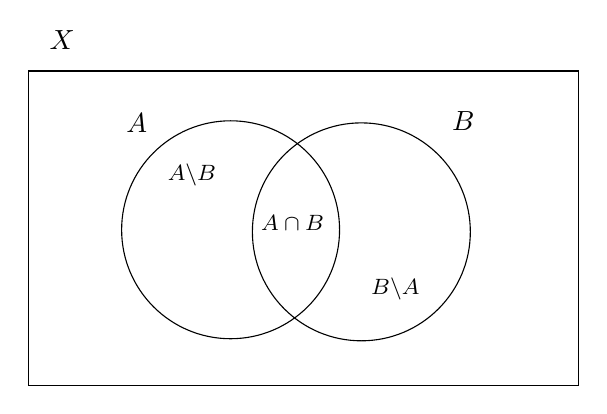
\begin{tikzpicture}[x=0.75pt,y=0.75pt,yscale=-1,xscale=1]
%uncomment if require: \path (0,224); %set diagram left start at 0, and has height of 224

%Shape: Circle [id:dp4825947291608632]
\draw  [color={rgb, 255:red, 0; green, 0; blue, 0 }  ,draw opacity=1 ] (242,131.5) .. controls (242,102.51) and (265.51,79) .. (294.5,79) .. controls (323.49,79) and (347,102.51) .. (347,131.5) .. controls (347,160.49) and (323.49,184) .. (294.5,184) .. controls (265.51,184) and (242,160.49) .. (242,131.5) -- cycle ;
%Shape: Circle [id:dp5232244089626727]
\draw   (305,132.5) .. controls (305,103.51) and (328.51,80) .. (357.5,80) .. controls (386.49,80) and (410,103.51) .. (410,132.5) .. controls (410,161.49) and (386.49,185) .. (357.5,185) .. controls (328.51,185) and (305,161.49) .. (305,132.5) -- cycle ;
%Shape: Rectangle [id:dp8863905853558256]
\draw   (197,55) -- (462,55) -- (462,206.43) -- (197,206.43) -- cycle ;

% Text Node
\draw (206,34.4) node [anchor=north west][inner sep=0.75pt]    {$X$};
% Text Node
\draw (243,74.4) node [anchor=north west][inner sep=0.75pt]    {$A$};
% Text Node
\draw (400,73.4) node [anchor=north west][inner sep=0.75pt]    {$B$};
% Text Node
\draw (263,98.4) node [anchor=north west][inner sep=0.75pt]  [font=\footnotesize]  {$A\backslash B$};
% Text Node
\draw (308,123.4) node [anchor=north west][inner sep=0.75pt]  [font=\footnotesize]  {$A\cap B$};
% Text Node
\draw (361,153.4) node [anchor=north west][inner sep=0.75pt]  [font=\footnotesize]  {$B\backslash A$};

\end{tikzpicture}
\end{figure}
\\
\begin{lemma}{ }
    \begin{itemize}
        \item[(i)] $X \cup Y = Y \cup X$, $X \cap Y = Y \cap X$ (Commutativity)
        \item[(ii)] $X \cup (Y \cup Z) = (X \cup Y) \cup Z$, $X \cap (Y \cap Z) = (X \cap Y) \cap Z$ (Associativity)
        \item[(iii)] $X \cup (Y \cap Z) = (X \cup Y) \cap (X \cup Z)$, $X \cap (Y \cup Z) = (X \cap Y) \cup (X \cap Z)$ (Distributivity)
    \end{itemize}
\end{lemma}
To prove it rigorously, we need apply the definition of the equality of two sets, which is definition \textbf{2.1.5}.
Here we are only going to prove the first equality. $\forall x \in X \cup Y$, $x \in X \lor x \in Y \iff x \in Y \lor x \in X$, which means $x \in Y \cup X$, hence $X \cup Y \subseteq Y \cup X$. Applying the same method will result in $Y \cup X \subseteq X \cup Y$,
which implies that $X \cup Y = Y \cup X$.
\begin{defin}{Cartesian product}
    Suppose $X$, $Y$ are two sets, then \textbf{Cartesian product} of $X$, $Y$ are denoted by $X \times Y$,
    which is the set
    $$
    X \times Y = \{(x, y)\ |\ x\in X, y \in Y\}
    $$
\end{defin}
Two elements inside it are equal if and only if the elements in each component of the cartesian product are equal, i.e   $(a,a') = (b,b')$ if and only if $a = b$ and $a' = b'$.\\
\textbf{Proposition}\quad Let $X$ and $Y$ be sets,
$$X \times Y = \emptyset \iff (X = \emptyset) \lor (Y = \emptyset)$$
\textbf{Proof}:\\
To prove an if and only if statement, there are two directions for us to prove, let's first prove `$\implies$' one. Prove by contradiction,
suppose that $X \times Y = \emptyset$ but $(X \neq \emptyset) \land (Y \neq \emptyset)$. This means that $\exists\ x \in X, x = x$ and $\exists\ y \in Y, y = y$.
Now $\exists\ (x,y) \in X \times Y, (x, y) = (x, y)$. Therefore $X \times Y \neq \emptyset$.\\
Let's that prove backwards, `$\Longleftarrow$'. Prove by contrapositive, suppose $X \times Y \neq \emptyset$, then $\exists\ (x,y) \in X \times Y, (x, y) = (x, y)$, this means
that $\exists\ x \in X, x = x$ and $\exists\ y \in Y, y = y$, hence $(X \neq \emptyset) \land (y \neq \emptyset)$. \qed
\begin{defin}{Families if Sets}
    Let $A$ be a nonempty set, $\forall \alpha \in A$, let $A_{\alpha}$ be a set.
    $$
    \mathcal{A} \coloneqq \{A_{\alpha}\ |\ \alpha \in A \}
    $$
    is called a family of sets and $A$ is the index set for this family.
\end{defin}
Let $X$ be the universal set of all sets in the family set. Intersection and union of those sets will be denoted as below:
$$
\underset{\alpha}\bigcap\ A_{\alpha} \coloneqq \{x \in X \ |\ \forall \alpha \in A,\ x \in A_{\alpha} \}
$$
$$
\underset{\alpha}\bigcup\ A_{\alpha} \coloneqq \{x \in X\ |\ \exists \alpha \in A,\ x \in A_{\alpha}\}
$$
\quad\ \  Let $\{A_{\alpha}\ |\ \alpha \in A\}$ and $\{B_{\beta}\ |\ \beta \in B\}$ be families of subsets of a set $X$, then $ (\bigcap_{\alpha}A_{\alpha}) \cap ( \bigcap_{\beta} B_{\beta}) = \bigcap_{(\alpha, \beta)} A_{\alpha} \cap B_{\beta}$.\\
\textbf{Proof}:\\Let
$S_{l} = (\bigcap_{\alpha}A_{\alpha}) \cap ( \bigcap_{\beta} B_{\beta})$ and $S_{r} = \bigcap_{(\alpha, \beta)} A_{\alpha} \cap B_{\beta}$. $\forall x \in S_{l}$, we can see $x \in \bigcap_{\alpha}A_{\alpha}$ and $x \in \bigcap_{\beta} B_{\beta}$, meaning
$\forall \alpha \in A$ and $\forall \beta \in B$, $x \in A_{\alpha}$ and $x \in B_{\beta}$. Thus, $\forall (\alpha, \beta) \in A\times B$, $x \in A_{\alpha} \cap B_{\beta}$, which means $x \in S_{r}$. Similarly, if $x \in S_{r}$, then $\forall (\alpha, \beta) \in A \times B$,
$x \in A_{\alpha}\cap B_{\beta}$. Fix $\beta$, running through $A$ for $\alpha$, $x \in \bigcap_{\alpha} A_{\alpha}$, similarly, $x \in \bigcap_{\beta} B_{\beta}$. \qed\\
There are also some interesting things to consider about if we consider the following \textbf{Proposition},
$$
\left(\bigcap_{\alpha}A_{\alpha}\right) \times \left( \bigcap_{\beta} B_{\beta}\right) = \bigcap_{(\alpha, \beta)} A_{\alpha} \times B_{\beta}
$$
\textbf{Proof}:\\
Very similar method to what we have applied before except decomposing an element into two components. \qed\\
\textbf{Distributivity} and \textbf{de Morgan's law} are also true in family of sets.
\begin{itemize}
    \item{distributivity}
    \begin{center}
        $(\bigcap_{\alpha}A_{\alpha}) \cup ( \bigcap_{\beta} B_{\beta}) = \bigcap_{(\alpha, \beta)} A_{\alpha} \cup B_{\beta}$\\
        $ (\bigcup_{\alpha}A_{\alpha}) \cap ( \bigcup_{\beta} B_{\beta}) = \bigcup_{(\alpha, \beta)} A_{\alpha} \cap B_{\beta}$
    \end{center}
    \item{de Morgan's law}
    \begin{center}
                        $(\bigcap_{\alpha}A_{\alpha})^c = \bigcup_{\alpha} A_{\alpha} ^ c$\\
                        $(\bigcup_{\alpha}A_{\alpha})^c = \bigcap_{\alpha} A_{\alpha} ^ c$
    \end{center}
\end{itemize}
Let's prove the first one and the forth one to give an example and basic idea.\\
\textbf{Proof}:(First One)\\
Denote right hand side as $S_r$ and left hand side as $S_l$. $\forall x \in S_r$, $x \in \bigcap_{\alpha} A_\alpha $ or $x \in \bigcap_\beta B_\beta$, if $x \in \bigcap_\alpha A_\alpha$, then $x \in A_\alpha$ for all $\alpha$.
Thus $\forall (\alpha, \beta) \in A \times B$, we have $x \in A_\alpha \cup B_\beta$, $x \in S_r$, the other case is same as this case. Now let's pick any element from $S_r$,
%%%%%%%%%%%%%%%%%%%%%%%%%%%%%%%%%%%%%%%%%%%%%%%%%%%%%%%%%%%%%%%%%%%%%%%%%%%%%%%%%%%%%%%%%%%%%%%%%%%%%%%%%%%%%%%%%%%%%%%%%%%
\newpage
\section{Groups}
\subsection{Operations}
\begin{defin}{Operation}
    A function $\odot : X \times X \rightarrow X$ is called an operation on $X$.
\end{defin}
To be convenient, we write $x\odot y$ instead of $\odot(x,y)$. For nonempty subsets $A$ and $B$ of $X$, denoting $A \odot B$ as:
$$
A \odot B = \{a \odot b\ |\ a \in A,\ b \in B\}
$$
\quad\ A nonempty subset $A$ of $X$ is \textbf{closed under the operation} if $A \odot A \subseteq A$. For example, let $\odot$ be
$+$ in $\mathbb{R}$. Now $\mathbb{N}$ is closed under the operation.
\begin{defin}{Associative}
    An operation $\odot$ on $X$ is associative if
    $$
    \forall\ x, y, z \in X,\  x \odot (y \odot z) = (x \odot y) \odot z
    $$
\end{defin}
Pick the previous example here, we can see $+$ on $\mathbb{N}$ is associative. It is not hard to find some operations that are not associative
since you can define operation as whatever you like. Consider the following example, let $X = \mathbb{N} \times \mathbb{N}$, define $\odot$
to be a function from $\mathbb{N}^2 \times \mathbb{N}^2 \rightarrow \mathbb{N}^2$ as following: $(a_1, b_1) \odot (a_2, b_2) = (a_1 + a_2, b_1 + b_2)$
if $a_1 + a_2 = 1$, otherwise, define it to be $(a_1 + a_2, b_1 + b_2)$. Consider $(1,\ 0)\odot \left((0,\ 1) \odot (2,\ 3)\right)$ and $\left((1,\ 0)\odot (0,\ 1)\right)\odot (2,\ 3)$.
The previous one is equal to $(3,\ 4)$ while the second one is equal to $(2,\ 3)$.
\begin{defin}{Commutative}
    An operation $\odot$ on $X$ is commutative if
    $$
    x \odot y = y \odot x
    $$
    $\forall x,\ y \in X$, i.e. given any two elements in $X$.
\end{defin}
The bracket matters when multiple operations taken in the same time, we should ask a question for ourselves, will they come out for the same result? Or they will have different
result depending on how we put the bracket?\\

Don't be confused that in the following theorem, the parentheses have the same meaning as brackets.
\begin{thm}{Arbitrary parentheses}
    Let $\odot$ be an associative operation on a set $X$. Then the value of any valid expression only involving $\odot$, elements of $X$ and parentheses,
is independent of the placement of the parentheses.\\
\textbf{Proof:}\\
One can define the result of one way recursively. Let $K_1 \coloneqq a_1$ and $K_{n+1} = K_n \odot a_{n+1}$. Now $K_n$ is something like
$$
(\cdots((a_1 \odot a_2)\odot a_3)\odot \cdots)\odot a_{n-1})\odot a_n
$$
Denote any expression with length $n$ to be $A_n$. The thing left for us is to prove that $A_n = K_n$. By definition of associative operation, we know that
$A_3 = K_3$ and there is nothing to prove for $n = 2$ or $n = 1$. For $A_{n+1}$, by considering the last operation it should take, it can must be written as $A_l \odot A_m$,
where $m + l = n + 1$.
\begin{itemize}
    \item{Case 1}\\
     $m = 1$, now $A_{n+1} = A_n \odot a_{n+1}$. By induction, we know $A_n = K_n$, and because $K_{n+1} = K_n \odot a_{n+1}$, this tells us that $A_{n+1} =K_{n+1}$.
    \item{Case 2}\\
     $m > 1$, by induction, $A_m$ has the form $A_{m-1} \odot a_{n+1}$. This gives that $A_{n+1} = A_l \odot A_m = A_l \odot (A_{m-1} \odot a_{n+1})=$\footnote{Prove this equality by your own}$(A_l \odot A_{m-1})\odot a_{n+1}$.
     Since $A_l \odot A_{m-1} = A_{l+m-1} = K_{n}$. Hence $A_{n+1} = K_{n+1}$.
\end{itemize}
We finish this proof by claiming again that we make use of induction to prove this theorem.
\qed
\end{thm}
To simplify how we write the expression, an expression of length $n$, is written as
$$
a_1 \odot a_2 \odot \cdots \odot a_n
$$
Without any parentheses.
\begin{defin}{Identity of an operation}
    Let $\odot$ be an operation on $X$. Any element $e$ of $X$ such that $\forall x \in X$
    $$
    e \odot x = x \odot e = x
    $$
is called an identity element.
\end{defin}
\begin{lemma}{Uniqueness of Identity}
    There is at most one identity element of one operation.
\end{lemma}
\subsection{Groups}
\begin{defin}{Group}
    A group is a nonempty set $G$ and an operation $\odot$ on $G$ with following properties hold:\\
    (G1) $\odot$ is associative.\\
    (G2) $\exists\ e \in G$, $\forall\ g \in G$, $e \odot g = g \odot e = g$.\\
    (G3) $\forall\ g \in G$, $\exists\ g^{-1} \in G$, such that $g \odot g^{-1} = g^{-1} \odot g = e$.
\end{defin}
When $\odot$ is commutative, we call such a group \textbf{Abelian} group. Here are some very basic properties of a group with some new definitions.
\begin{defin}{Order of a group}
    The \textbf{order} of a group $G$ is the number of elements it contains, usually denoted by $|G|$.

\end{defin}
If $|G|$ is finite, the group is called finite group, otherwise, it is called infinite group.
\begin{lemma}{Uniqueness of inverse}
    For every element $g \in G$, there exists a unique inverse, which is denoted by $g^{-1}$.\\
    \textbf{Proof}:\\
    Suppose $g_1$ and $g_2$ are both the inverses of $g$. Now
    $$
    g_1 = g_1 \odot e = g_1 \odot (g \odot g_2) = (g_1 \odot g) \odot g_2 = g_2
    $$
    where the second equality is obtained by G1.
    \qed

\end{lemma}
There are also some laws that you will be very familiar with when you are working with daily real number operations.
\begin{lemma}{Cancellation Law}
    Let $g_1$, $g_2$ and $g_3$ be elements of a group $G$, then
    $$
    g_1 \odot g_2 = g_1 \odot g_3 \implies g_2 = g_3
    $$
\end{lemma}
You can verify easily that if $g$, $h$ are elements of a group $G$, then
$$
(g \odot h)^{-1} = h^{-1} \odot g^{-1}
$$
\quad\ Below is a list of groups and they properties.
\begin{itemize}
    \item The $n \times n$ general linear group. This is the group of all invertible $n \times n$ matrices. And it is denoted by
    $$GL_n = \{n \times n \text{ invertible matrices }A\}$$
    \item The group of permutations of the set of indices $\{\mathbf{1, 2, \cdots, n}\}$ is called symmetric group, denoted by $S_n$.
    \item The set of integers with addition $+$, denoted by $\mathbb{Z}^+$.
\end{itemize}
\section{The Sylow Theorems}
\subsection{Statements of Three Theorems}
These are notes taken from the book Algebra written by Artin. A Sylow $p$-subgroups is a $p$ group which is a subgroup of that group whose
index is not divisible by $p$.
\begin{thm}{First Sylow Theorem}
    A finite group whose order is divisible by a prime $p$ contains a Sylow $p$-subgroup.
\end{thm}
Apply this theorem, we obtain following Corollary. A finite group whose order is divisible by $p$ contains an element of order $p$. This 
can be proved by following argument: call this group $G$, then it contains a Sylow $p$-subgroup. Pick an element $x$ which is different from identity, 
its order must be positive power of $p$. Suppose it's $p^k$, then $x^{k -1}$ has order $p$.
\begin{thm}{Second Sylow Theorem}
    Let $G$ be a finite group whose order is divisible by a prime $p$.
    \begin{itemize}
        \item The Sylow $p$-subgorups of G are conjugate subgroups
        \item Every subgroup of $G$ that is a $p$-group is contained in a Sylow $p$-subgroup.
    \end{itemize}
\end{thm}
The first point of this theorem is to say that, given $G_1, G_2 \unlhd G$, there exists $g \in G$, s.t. $G_1 = g G_2 g^{-1}$. Additionally, given a Sylow $p$-subgroup $H$
of $G$, $\forall g \in G$, $g H g^{-1}$ is also a Sylow $p$-subgroup. 
\begin{thm}{Third Sylow Theorem}
    Let $G$ be a finite group whose order $n$ is divisible by a prime $p$. Given that $n = p^e m$ where $m$ is not divisible by $p$. Then if $s$ is the number of Sylow $p$-subgroup, 
   then $s | m$ and $s \equiv 1$ (mod $p$).
\end{thm}
The Third theorem is very strong so that it can help us to classify some groups whose order are not large enough. The things left to do is to prove those three theorems.
\subsection{Preparation of Proofs}
Before proving those theorems, let's first introduce a simple group action. Suppose that $G$ acts on set $S$. Given a subset $U$ of $S$, define
$$
gU \coloneqq \{gu\ |\ u \in U\}
$$
One can easily verify that $|gU| = |U|$. Hence if we pick all the subsets of $G$ with order $|U|$, G acts on this set with operation defined as $(g, U)\mapsto gU$. Axioms for group action
 can be checked easily.
\begin{lemma}{ }
$G$ is a group and $U \subseteq G$. If $G$ acts on the set of all subsets of $G$ with order $|U|$ by left multiplication, then $|\text{Stab}(U)|$ divides both $|U|$ and $|G|$.
\end{lemma}
By counting formula $|\text{Stab}(U)| |O_U| = |G|$, therefore the second divisibility is trivial. To prove the first one, we should define a relation of $U$ where 
$$
R(u_1,u_2)\Longleftrightarrow u_1 \in \text{Stab}(U) u_2
$$
By checking reflexive, symmetry and transitivity, it can be proved that this is an equivalence relation. By some simple implications, the first divisibility can be proved.
\begin{lemma}{ }
Let $n$ be an integer of form $p^{e}m$, where $e > 0$ and $p$ does not divide $m$. The number $N$ of subsets of order $p^{e}$ in a set of order $n$ is not divisible by $p$.
\end{lemma}
This is simply a number theory problem, since we can directly calculate the number $N$, which is 
$$
\frac{n(n-1)\cdots(n-k)\cdots(n - p^e + 1)}{p^e (p^e - 1)\cdots (p^e - k) \cdots 1}
$$
Let's prove by contradiction that this number is not divisible by $p$. Suppose it's divisible by $p$, then 
$$
\frac{n(n-1)\cdots(n-k)\cdots(n - p^e + 1)}{p^e (p^e - 1)\cdots (p^e - k) \cdots 1} = p q
$$
where $q$ is an arbitrary natural number which is not $0$. Hence
$$
n(n-1)\cdots(n-k)\cdots(n - p^e + 1) = p^e (p^e - 1)\cdots (p^e - k) \cdots 1 \cdot p \cdot q
$$
Conisder the term $n - k = p^e m - k$, if $k$ is not divisible by $p$, then $n-k$ is not divisible by $p$. Thus, suppose we pick 
all the $k$s where $k$ is divisible by $p$. $k$ can be written as $p^{k_i} \cdot l$. Since $k_i < e$, $n - k$ is divisible by $p^{k_i}$ but not 
$p^{k_i + 1}$. So left hand side is divisible by $\sum_{\text{all }k} k_i$ but not $\sum_{\text{all }k} k_i + 1$. However right hand side is divisible by 
$\sum_{\text{all }k} k_i + 1$ because $p^e - k = p^e - p^{k_i} \cdot l$, which is divisible by $p^{k_i}$. Contradiction!
\subsection{Proof of The Sylow's Theorems}
Proof of the first Sylow's Theorem: Let's recall the first theorem needs to prove that a group $G$ with order $n = p^e m, e > 0$ must have a Sylow $p$-subgroup, which 
is just a subgroup of order $p^e$. This construction is not straightforward, picking set $S$ which consists of subsets of $G$ of order $p^e$. We know orbits partition set
$S$, so
$$
|S| = \sum_{\text{orbits } O} |O|
$$
According to lemma 4.2.2, $|S|$ is not divisible by $p$. This means at least one orbit's order is not divisible by $p$. Call this subset $U$, now $|\text{Stab}(U)|$ divides $|U|$, $|\text{Stab}(U)|$ 
must be some positive power of $p$. Since $|O_U|$ is not divisible by $p$, the only possibility is that $|O_U| = m$ and $|\text{Stab}(U)| = p^e$. \qed\\
Proof of Sylow's Second Theorem: Suppose there is a $p$-subgroup $K$. The equivalent statement of Sylow's Second Theorem is that, given a Sylow $p$-subgroup $H$, there exists $g \in G$, such that $K \subseteq g H g^{-1}$.
Construct a set $\mathcal{C}$ for which $G$ acts on which has the folloing properties. $p$ does not divide $|\mathcal{C}|$ and $\exists\ c \in \mathcal{C}$ such that $\text{Stab}(c) = H$. The existence of this set can be 
proved easily since that the set of left cosets of $H$ is one of examples. Since the order of this set is $m$ and $\text{Stab}(H) = H$. Additionally, the action is transitive.
Now restrict our action for only $K$, then there must exists $c' \in \mathcal{C}$ which $c'$ is a fixed point. That is $k(c') = c'$ for all $k \in K$. This meaning $K \subseteq \text{Stab}(c')$. $c' = g(c)$, meaning $\text{Stab}(c') = g \text{Stab}(c) g^{-1}$.
\qed\\
Proof of Sylow's Third Theorem: Use the symbols in our statement of the third Sylow's Theorem. Let $S$ be the set of all the Sylow $p$-subgroup. Now $G$ acts on $S$ by conjugation. Moreover, we know that this action is transitive by 
Second Sylow's Theorem. Pick one particular Sylow $p$-subgroup $H$. Call its stabilizer $N = N(H)$. By counting formula, $|G| = |N||O_{H}| = |N||S|$. Since $H \subseteq N$, then $|H| | |N|$ as $H$ is a subgroup of $N$. Using those two identities, you can actually
deduce $s | m$. Now let's prove the second identity, where we focus on the group action of $H$ on $S$. The orbit of $H$ is just itself because $H$ will be fixed by any element from $H$ by conjugation. Any other set who is not fixed by $H$ will have orbit of order 
greater than $2$, and the order divides a positive power of $p$. Therefore we only need to prove the only set that is fixed by $H$ is $H$ itself. Suppose that there is another set $H'$ which is fixed by $H$. 
Then the normalizer $N'$ of $H'$ contains $H$ and $H'$ as Sylow $p$-subgroups. $\exists\ n \in N$, such that $n H' n^{-1} = H$, however $H'$ is normal in $N'$. Thus, $H = H'$. \qed
\end{document}